
%\begin{itemize}
%\item mini seccion que repita idea
%\item seccion que describe la arquitectura y cada modulo.
%\item aspectos de implementacion (resumidos) 
%\item seccion que muestra un ejemplo de programación.
%\end{itemize}

%En esta secci\'on describiremos la arquitectura de la interfaz ERBPI. 
%Para el dise\~no de la misma, hemos decidido optar por un dise\~no modular que brinde responsabilidades claras y delimitadas en los m\'odulos, donde una modificaci\'on en un m\'odulo impacte lo menos posible en el resto de la aplicaci\'on, y que al mismo tiempo nos brinde tambi\'en la posibilidad de extensibilidad de caracter\'isticas de la aplicaci\'on, dandole  la capacidad de adaptarse a los cambios de requerimientos, pudiendo ser extendida con facilidad, sin la necesidad de sufrir modificaciones. Hasta este momento hemos implementado los distintos m\'odulos que componen la aplicaci\'on y que detallaremos m\'as adelante: CORE, RAL y GUI. Nos queda pendiente aun realizar la implementaci\'on del feature de subsumici\'on.
 

%Como dijimos anteriormente, la interfaz de programaci\'on de robots ERBPI utiliza el paradigma conexionista para programar los comportamientos del robot. La aplicaci\'on permite al usuario establecer conexiones entre los distintos sensores y actuadores del robot. Cada conexi\'on puede ejecutar una funci\'on matem\'atica dando lugar a un grafo de ejecuci\'on that perform the basic behaviour (Fig. \ref{Fig:grafo})

ERBPI uses a behaviour-based approach following the connectionist paradigm. It enables users to create basic behaviours, and then connect them using a subsumption architecture to create more complex ones. 

To create basic behaviours, the user establishes connections between sensors and actuators, and configures them with a chain of mathematical functions.  Each function can have several inputs, including sensed data and outputs from previous ones. It uses all the inputs to compute a single output, that in turn may be used to set actuators or input following functions. The user chooses functions from predefined families and configure their parameters. %This output may be used to set one or more actuators, or to input a following function. 
This schema defines an execution graph that allows to infer a computation order and thus translate it to an imperative program for the robot. 

%\begin{figure}
% \centering
% 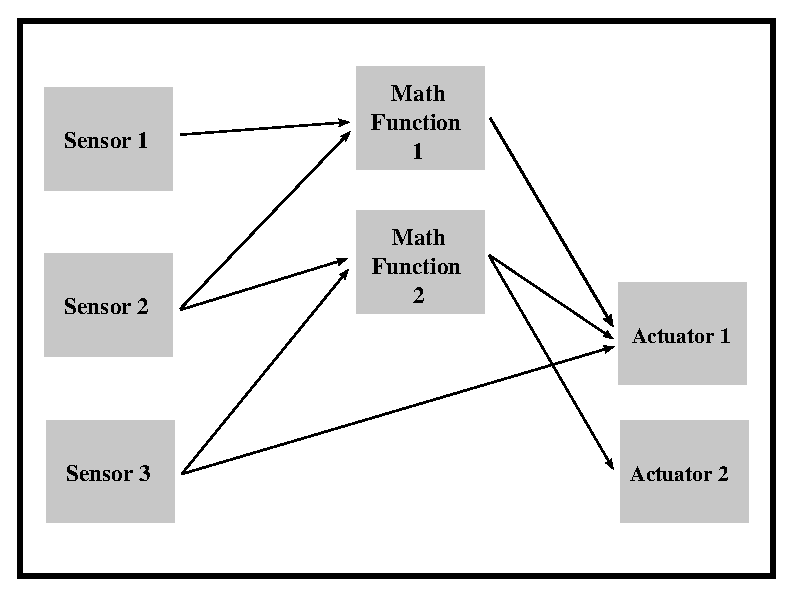
\includegraphics[scale=0.5]{images/grafo_eng.eps}
% \caption{An example of execution graph.}
% \label{Fig:grafo}
%\end{figure}

All the function outputs, sensors and actuators values are normalized to the same scale ($-100, 100$). This scale is a ``percentage of activation'' for each element in the schema. Normalizing all the data permits the previous schema to work properly and also that one behaviour can be used for several robots that may have different sensors or actuators. %The translation of this normalized values to actual sensors or actuators values is performed by a particular robot abstraction layer, explained in section \ref{sec:RAL}.

%Different basic behaviours can be connected using a subsumision architecture, making it possible to achieve more complex behaviours. In this way, we get a state automaton, where each state represents a behaviour and each transition a change in the environment. This state machine can be easily translated into an imperative program that the robot executes to perform the behaviour.

The application has a modular design, clearly decoupling the different responsibilities in the system. The GUI (Graphical User Interface) module allows the user to graphically design the robot behaviour, and then exports this behaviour in a file. The CORE module reads this file and executes the defined behaviour. To communicate with the robotic platform (simulator or real robot), the CORE uses a particular RAL (Robot Abstraction Layer) module. There is one RAL for each robotic platform ERBPI manages. This module is in charge of normalizing all the sensor and actuator values, and also of communicating with the actual robot using its particular communication protocol. The basic architecture, including the three modules and their communication, is shown in Fig. \ref{Fig:arquitectura}. Each module is explained in the following sections. 

%La idea general de esta arquitectura es que mediante el m\'odulo GUI el usuario pueda programar el comportamiento del robot de forma gr\'afica y sensilla. Una vez hecho esto, el comportamiento es entregado al m\'odulo CORE que se encarga de ejecutar el comportamiento, utilizando el módulo m\'odulo RAL, que ser\'a el encargado de establecer la conexi\'on entre el CORE y el robot correspondiente.

%Es importante tener en cuenta, como dijimos antes, que hemos dado a la aplicaci\'on la capacidad de poder ser extendida en muchas de sus caracter\'isticas sin la necesidad de ser modificada. Para esto, como veremos m\'as adelante, junto al dise\~no modular se utilizar\'an est\'andares de intercambio de informaci\'on, como XML (Extensible Markup Language), que permitir\'an tanto la comunicaci\'on entre los m\'odulos como la configuraci\'on de los mismos y de toda la aplicaci\'on, features setting, agregar robots, modificar caracter\'isticas de los robots, etc. 

%En la Fig. \ref{Fig:arquitectura} podemos ver la arquitectura de la aplicaci\'on, con sus tres m\'odulos y la comunicaci\'on entre ellos. A continuación vamos a explicar cada módulo en detalle.

\begin{figure}
 \centering
 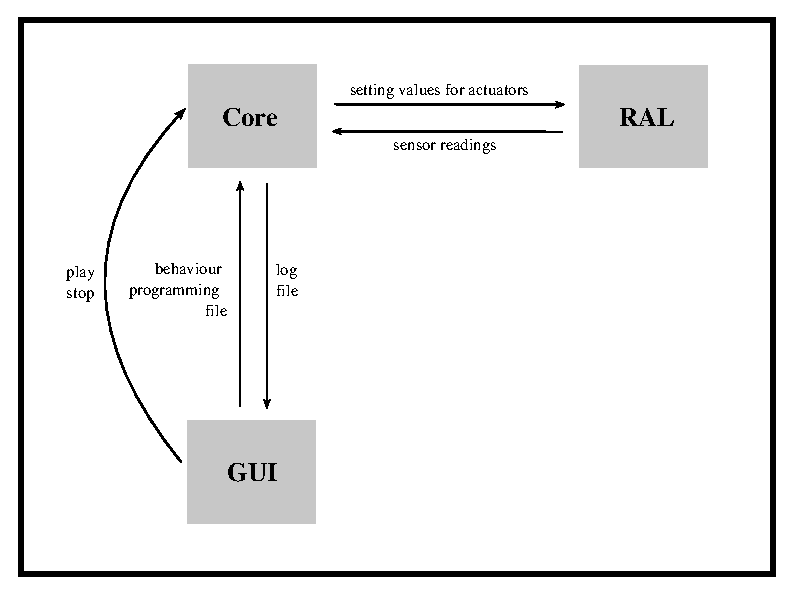
\includegraphics[scale=0.7]{images/arq_eng.eps}
 \caption{ERBPI's modular architecture.}
 \label{Fig:arquitectura}
\end{figure}

\subsection{GUI (Graphical User Interface) Module}

The GUI module is in charge of interacting with the user. To start, the user selects a robot or simulator to work with. The GUI enables the user to drag and drop elements (sensors, actuators, functions) to a work canvas, and then connect them using the mouse. Different functions may be selected from a menu, dragged to the canvas, and then configured with a pop-up configuration window. Fig. \ref{Fig:guiCanvas} shows a screenshot of the GUI and Fig. \ref{Fig:guiFunction} an example of the pop-up configuration window. 

%El módulo GUI (Graphical User Interface) se encarga de la interfaz con el usuario. Primero debemos seleccionar con qué robot (o silumador) queremos trabajar. Luego seleccionamos los sensores y actuadores del robot que vamos a usar para el comportamiento que queremos hacer. Mediante mecanismos muy sencillos de arrastrar y soltar (drag-and-drop) los diferentes objetos (sensores, actuadores, conexiones) en un escritorio de trabajo, podremos generar diferentes comportamientos. Cada conexión sensor-actuador posee una ventana emergente que permite definir funciones matemáticas parametrizables. De esta forma, el usuario construye un grafo de ejecución que representa el comportamiento a realizar, donde los nodos son los sensores, actuadores y funciones matemáticas, como podemos apreciar en la Fig. \ref{Fig:gui01} 

\begin{figure}
 \centering
 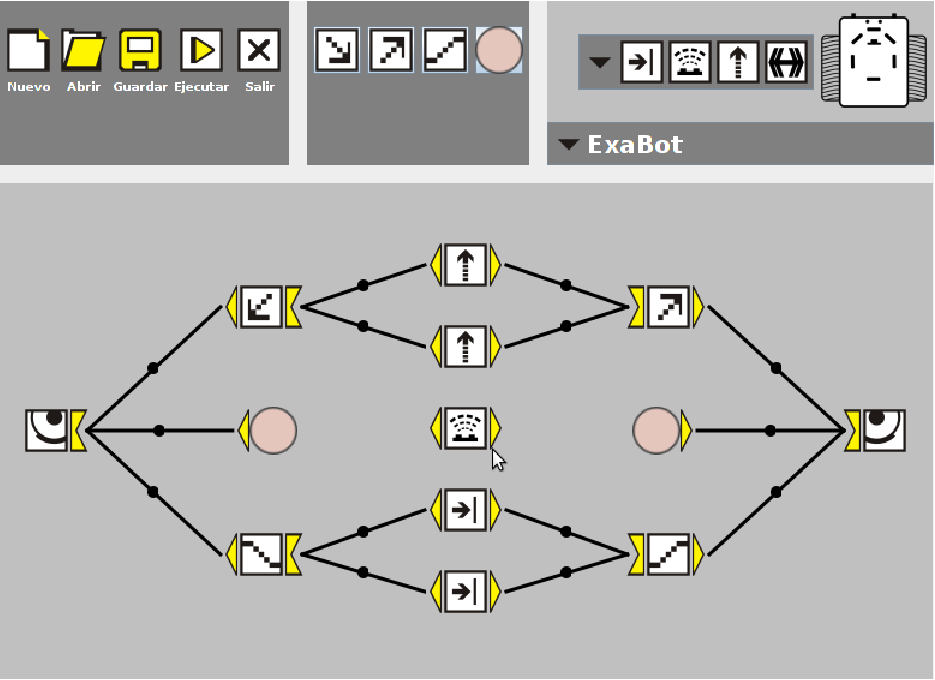
\includegraphics[scale=0.3]{images/gui_canvas.png}
 \caption{A screenshot of the application. The upper panel shows the configurations and elements. The general operations (new, open, save, play, quit) are in the upper left corner. The upper-center panel has different families of functions the user can choose from (decreasing, growing, broken and constant functions in this screenshot). The upper right panel shows the selected robot with its sensors. In the canvas we can see a line following behaviour that stops when the bumpers are activated.}
 \label{Fig:guiCanvas}
\end{figure}

\begin{figure}
 \centering
 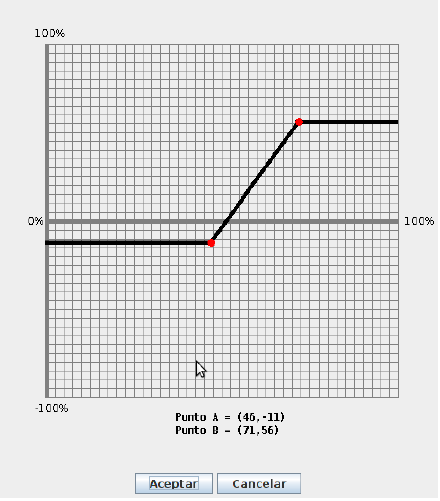
\includegraphics[scale=0.3]{images/gui_function.png}
 \caption{The configuration pop-up window for a broken function. The change points in the function and the low and high levels can be easily configured moving them with the mouse. The scale for the normalized values ($-100, 100$) is also observable. }
 \label{Fig:guiFunction}
\end{figure}
%Otra caracter�stica importante del m�dulo GUI es que tiene la funci�n de ser la interfaz gr�fica de la aplicaci�n completa, coordinando el funcionamiento de los distintos m�dulos. De esta forma, 

Once the behaviour is finished, the user can select a robot to execute it on. The created behaviour and the minimal sensor and actuator configuration needed for its execution are stored in a file (the behaviour-file), that will be read by the CORE. The execution of the behaviour may be started and paused at any moment from the GUI. The GUI also provides general operations to open and save files. 

The GUI is implemented in Java, a good language for graphical interfaces and portable to several operating systems, only requiring the installation of the JVM (Java Virtul Machine). The behaviour-file is in XML(Extensible Markup Language), making it very simple to add new robots, sensor types, functions and other features we might add to ERBPI. A simple example of a behaviour-file is shown in table \ref{xml}. 


\begin{table}[ht!]
\footnotesize
\begin{Verbatim}[frame=single]
     <behaviour> 
       <sensors>
         <sensor id='sonar.0'/>
         <sensor id='encoder.motor.left'/>
       </sensors>
       <functions>
         <function id='function1'>
           <inputs>
             <input id='sonar.0'/>
             <input id='encoder.motor.left'/>
           </inputs>
           <points>
             <point x='100' y='0'/>
             <point x='150' y='255'/>
           </points>
         </function>
       </functions>
       <actuators>
         <actuator id='motor.left'>
           <inputs>
             <input id='function1'/>
             <input id='function2'/>
           </inputs>
         </actuator>
       </actuators>
     </behaviour>
\end{Verbatim}
\normalsize
\caption{Example of an XML behaviour-file. In this case, two sensors are needed to perform this behaviour (a sonar and an encoder). A broken function (\texttt{function1}), defined by two points, takes both sensors as inputs. The value for the motor.left actuator is set by the output of two functions}
\label{xml}
\end{table}

%En este caso hemos utilizado el lenguaje de programación Java para la implementacion. Hemos realizado esta elección por la capacidad de portabilidad de este lenguaje y la no necesidad de recompilar para distintos Sistemas Operativos.

%Una vez creado el comportamiento para el robot, podemos indicar sobre cuál robot se ejecutará. %y ejecutarlo con tan s�lo presionar \textit{play} en la GUI. 
%El comportamiento creado y la configuración de sensores y actuadores requerida para el robot en cuestión se guardan en un archivo de configuración que es entregado al múdulo CORE para su ejecución. La ejecución del comportamiento puede iniciarse y pausarse en cualquier momento también desde la GUI. Además la interface tiene botones para guardar el comportamiento en cuestión o abrir otro generado previamente.

\subsection{CORE module}

The CORE module is in charge of executing the behaviour. It reads the XML behaviour-file and establishes a connection with the appropriate RAL. At regular intervals, the core receives from the RAL the normalized values of the sensors, executes the behaviour, and gives to the RAL the normalized values to set the actuators. The CORE stops when the GUI signals the user has stopped the execution. 

To be able to execute the behaviour, the CORE has to transform the execution graph defined by the GUI in the behaviour-file to a corresponding ordered execution list, to guarantee that all the inputs for a function are ready when its turn to execute is up. For this, we used a topological sorting \cite{topologicalSorting} of the execution graph. The CORE also asserts that the behaviour can be executed in the selected robot, for example that the graph is not cyclic (i.e, cannot be ordered) or that the robot has enough sensors and actuators to execute the behaviour. It also defines the communication frequency with the RAL depending on the robots working frequency. Finally, the CORE makes a log-file where all the values at a certain time are registered, including each sensor value, the output value of each function and the value of each actuator. This log file is communicated to the GUI. We plan to use it to implement a debug function in the future. 


%El modulo CORE es el encargado de leer el archivo de comportamiento y ejecutarlo. Para esto, debe establecer una conexión con el múdulo RAL (Robot Abstraction Layer), le envia comandos para los actuadores del robot y recibe del RAL el estado del robot. Otra tarea del CORE es realizar una serie de chequeos correspondientes a la factibilidad de ejecución de ese comportamiento en el robot indicado. Por ejemplo, si el comportamiento definido por el usuario da lugar un gráfo acíclico que puede ser ejecutado secuencialmente, o si el robot posee los sensores y actuadores requeridos para llevar a cabo ese comportamiento. El módulo CORE también debe definir la frecuencia con la que se comunica con el RAL, dado que cada robot o simulador tiene una frecuencia de trabajo diferente dependiendo de sus unidades de procesamiento, sensores y actuadores. 
%Por último, el CORE lleva un registro de todo lo sucedido a traves de un archivo de \textit{log}, donde se deja registo del valor de cada sensor, de la función matemática que aplica en la conexión sensor-actuador y del valor actuador a cada momento, y que comunica a la GUI para poder realizar \textit{debug} del comportamiento del robot.

\subsection{RAL (Robot Abstraction Layer) module}
\label{sec:RAL}

The RAL modules encapsulates all the knowledge of the particular robot or simulator, providing a standard interface to the CORE module, dealing with everything necessary to communicate with the actual robot. The RAL abstracts the particular robot, its communication protocol, and normalizes the values of the particular sensors and actuators. In this way, all the specific characteristics of the robot are transparent to the CORE. A RAL must implement a standard interface that include the following methods:  get the list of sensors and actuators in the robot, get the frequency the robot can work in, get the sensor values, and set the values for the actuators. To add a new robotic platform for ERBPI to work with, a developer must only program a particular RAL for the platform implementing the general RAL interface.

All RALs are implemented as dynamic libraries. In this manner, we can add new RALs without having to recompile the CORE or the GUI. Moreover, this allows the CORE to load a different RAL on runtime, without having to restart the application. This makes ERBPI easily extendable to control different robots.

To the date, we have implemented RALs for the Khepera \cite{khepera} and Exabot \cite{exabot} robots, and for the YAKS (Yet another Khepera Simulator) \cite{yaks} and the Player/Stage \cite{player} simulator. 

%Hasta el momento, hemos implementado los RALs de dos robots y dos simuladores de los que disponemos en nuestro laboratorio: Khepera robot, YAKS (Yet Another Khepera Simulator), ExaBot robot, Player/Stage simulator.

%El modulo RAL se encarga de la comunicacion entre el CORE y el robot (real o simulado). 
%Como la aplicacion está concebida para trabajar con una amplia gama de robots y simuladores, necesitamos una capa de abstraccion respecto del hardware específico donde se va a ejecutar el comportamiento, es decir, qué tipo de robot, qué cantidad y tipo de sensores y actuadores, que tipo de comunicacion se utilizada para la conexion con el robot, etc.
%Por lo tanto, la características específicas de cada robot son transparentes para el módulo CORE, que solo se comunicara con el RAL para obtener el estado del robot y enviar el nuevo valor para sus actuadores. Luego, sera el RAL el que se comunicara directamente con el robot (real o simulado) segun corresponda.

%El RAL contiene una serie de funciones para obtener la lista de sensores y el estado de los mismos, obtener la lista de actuadores y setear el estado de los mismos y obtener la frecuencia de trabajo del robot.

%Para agregar un nuevo robot para trabajar con la aplicacion, solo deberemos programar el nuevo RAL correspondiente de ese robot e indicarle a la GUI en su archivo de configuración la existencia del nuevo robot.

%\subsection{Implementation issues}

%ERBPI is an open source project, so we used all open source libraries. We also used standard programming languages that 
%Hemos decidido realizar el desarrollo de la aplicación siguiendo los lineamientos de Software Libre, dando la libertad a los usuarios de la aplicacion para ejecutar, copiar, distribuir, estudiar, cambiar y mejorar el software. Siguiendo el mismo enfoque, y como pretendemos la mayor portabilidad posible de la aplicación a distintos ambitos (talleres en escuelas, charlas y demostraciones en diferentes instituciones, etc), también elegimos lenguajes de programacion estandares que puedan ser compilados y ejecutados en los sistemas operativos mas comunes como Windows o Linux. A continuación, detallaremos la implementación de cada módulo de la aplicación.

%\subsubsection{CORE}
%
%Lo hemos implementado en ANSI C++. Elegimos este lenguaje debido a que requerimos que la comunicacion con el robot sea lo mas cercana posible al tiempo real, y por lo tanto, que su ejecución sea también lo más rápida posible.

%\subsubsection{RAL}
%
%Como ya dijimos, es el encargado de la comunicacion efectiva con el robot, y por lo tanto, una manera sencilla de resolver esto es teniendo una implementacion distinta y particular para cada robot. El RAL también fue implementado en ANSI C++ por las mismas razones mencionadas anteriormente para el módulo CORE. En particular, hemos implementado el RAL como una libreria dinamica del sistema operativo. Esto nos permite cambiar el RAL específico para un robot en tiempo de ejecucion (runtime) de la aplicación. De esta forma, si bien existen distintas implementaciones del RAL para cada robot, éstas son transparentes al usuario de la aplicación, ya que es el CORE y la GUI, en runtime, los encargados de elegir la implementacion correspondiente para el robot elegido por el usuario. Esta última característica es la que permite extender la aplicación y trabajar con nuevos robots sin la necesidad de modificarla o recompilarla, lo único que se requiere es implementar el RAL correspondiente para el nuevo robot.
%
%Hasta el momento, hemos implementado los RALs de dos robots y dos simuladores de los que disponemos en nuestro laboratorio: Khepera robot, YAKS (Yet Another Khepera Simulator), ExaBot robot, Player/Stage simulator.

%\subsubsection{GUI} 
%
%En este caso hemos utilizado el lenguaje de programación Java para la implementacion. Hemos realizado esta elección por la capacidad de portabilidad de este lenguaje y la no necesidad de recompilar para distintos Sistemas Operativos. %Hoy d�a podemos ejecutar esta aplicaci�n en cualquier computadora que simplemente tenga instalada la Java Virtual Machine - JVM. Cosa que es raro no encontrar en cualquier computadora hogare�a. Esto �ltimo nos da la capacidad de ejecutar la aplicaci�n sin requerimientos previos.

%\subsubsection{Behaviour File} 
%En este caso utilizamos el formato XML (Extensible Markup Language). Esto también nos da la posibilidad de que el comportamiento pueda ser más complejo en el futuro, agregar funciones matemáticas nuevas, etc. sin la necesidad de modificar la aplicacion. Para esto, basicamente se utilizan diferentes \textit{labels} que denotan las distintas entidades y los input-output de cada una. En el caso de las funciones matemáticas se especifica además los puntos que conforman las curva de la funcion. Un ejemplo sencillo de behaviour file puede ser el siguiente:

%\footnotesize
%\begin{verbatim}
%     <behaviour>
%       <sensors>
%         <sensor id='sonar.0'/>
%         <sensor id='encoder.motor.left'/>
%       </sensors>
%       <functions>
%         <function id='function1'>
%           <inputs>
%             <input id='sonar.0'/>
%             <input id='encoder.motor.left'/>
%           </inputs>
%           <points>
%             <point x='100' y='0'/>
%             <point x='150' y='255'/>
%           </points>
%         </function>
%       </functions>
%       <actuators>
%         <actuator id='motor.left'>
%           <inputs>
%             <input id='function1'/>
%             <input id='function2'/>
%           </inputs>
%         </actuator>
%       </actuators>
%     </behaviour>
%\end{verbatim}
%\normalsize


%\subsubsection{GUI Setting File} 
%
%También utilizamos XML para su implementacion. Esto nos da la posibilidad de extender características de la aplicación como tipo de sensores a manejar, características sobre los mismos, qué tipos de robots puede operar, etc. sin la necesidad de modificar la aplicacion. Como en el caso anterior, utilizamos \textit{labels} que denotan las distintas características de la aplicacion. Un ejemplo sencillo de GUI setting file puede ser:

%\begin{verbatim}
%FALTA !!!!
%FALTA !!!!
%FALTA !!!!
%FALTA !!!!
%\end{verbatim}

%\subsubsection{Log File} 
%En este caso, por una cuestion de sencillez, implementamos esto con un archivo \textit{comma separeted}. Este archivo simplemente consta de una primera linea con la especificacion de cada columna (TimeStamp, sensores, funciones matemáticas y actuadores) y las siguientes con los valores correspondientes a cada una según la frecuencia de trabajo que se encuentra definida por el módulo RAL. En el caso de las funciones matemáticas se detalla el valor de entrada y salida. Un ejemplo de log file luego de la ejecucion de un comportamiento es:

%\footnotesize
%\begin{verbatim}
%timestamp, sonar.0, sonar.1, actuator.0, function.1, actuator.1,
%0, 6, 8, 8, 8, -9, 20,
%103, 3, 7, 7, 7, -8, 19,
%204, 8, 3, 3, 3, -6, 15,
%304, 7, 4, 4, 4, -6, 23,
%405, 7, 3, 3, 3, -6, 20,
%505, 10, 8, 8, 8, -9, 22,
%606, 4, 3, 3, 10, -6, 14,
%707, 3, 10, 10, 10, -13, 19,
%807, 8, 10, 10, 10, -13, 22,
%\end{verbatim}
%\normalsize
